\documentclass[12pt]{article}
\usepackage[letterpaper, margin=1in, headheight=105pt]{geometry}
\usepackage{subcaption}
\usepackage{graphicx}
\usepackage{hyperref}
\usepackage{pdfpages}
\usepackage{amsmath}
\usepackage{amssymb}
\usepackage{comment}
\usepackage{minted}
\usepackage{pgffor}
\usemintedstyle{manni}

\begin{document}
\setcounter{section}{2}
\begin{comment}
\section{Homework}
\subsection{Overfitting}
\begin{figure}[htbp]
    \centering
    \begin{subfigure}[t]{0.6\textwidth}
        \centering
        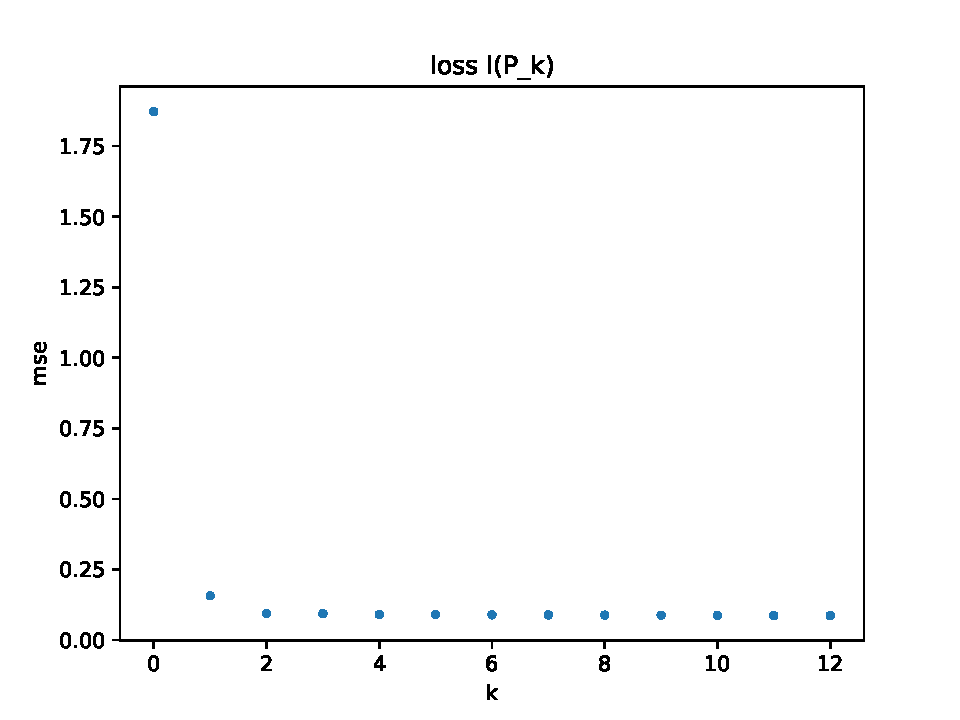
\includegraphics[width=\textwidth]{Homework1/ex1a.pdf}
        \caption{loss \(\ell(\hat{P}_k)\) as a function of \(k\)}
    \end{subfigure}\vspace{10pt}
    \begin{subfigure}[t]{0.6\textwidth}
        \centering
        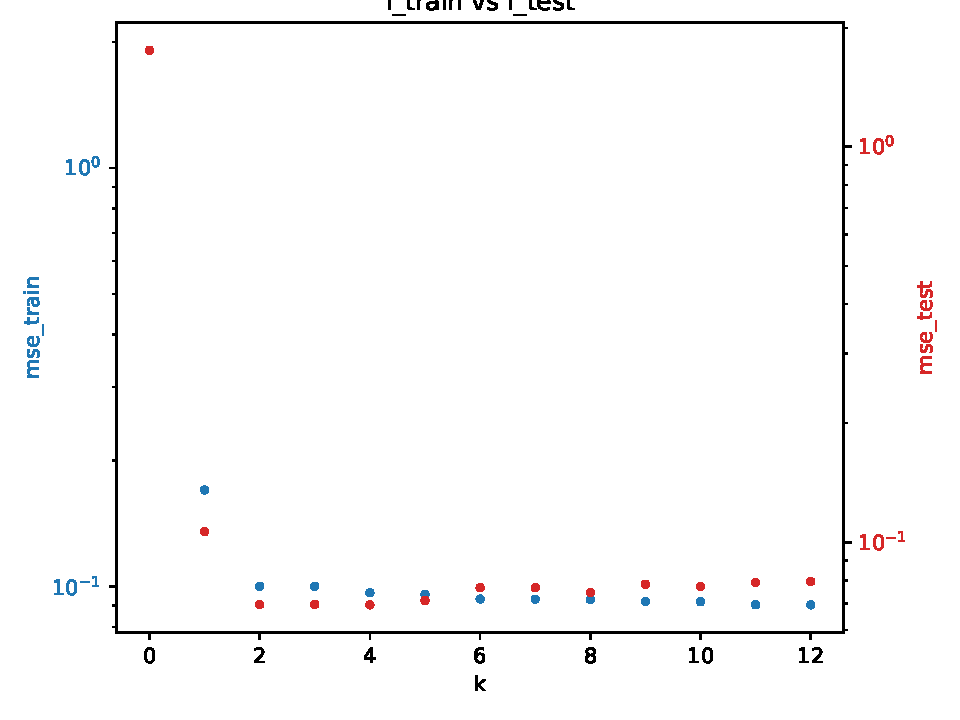
\includegraphics[width=\textwidth]{Homework1/ex1b.pdf}
        \caption{\(\ell_{train}(\hat{P}_k)\) vs \(\ell_{test}(\hat{P}_k)\)}
    \end{subfigure}
\end{figure}
By our observation, \(k_*=2\), and the coefficients are
\[ [a_0, a_1, a_2] = \begin{bmatrix} 0.35333775 & -0.27947762 & 0.81043897\end{bmatrix}. \]
\begin{figure}[htbp]
    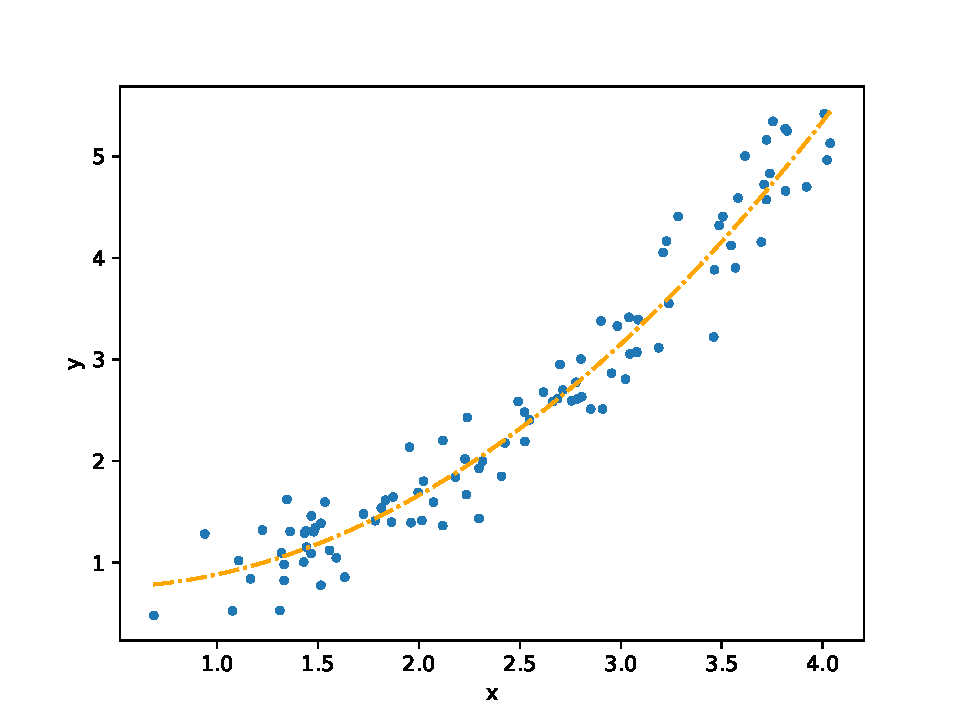
\includegraphics{Homework1/ex1c.pdf}
    \caption{Fitted polynomial by least-square linear regression}
\end{figure}
\inputminted[breaklines=true, linenos=true]{python}{./Homework1/ex1.py}
\newpage

\subsection{Gradient descent}
\paragraph{(a)}
The loss function can be expanded as
\[ \ell(a,b)= a^2 + b^2\overline{x^2}+ \overline{y^2} + 2ab\overline{x} - 2a\overline{y} - 2b \overline{xy} \]
The gradient of the loss functioin is
\[ \nabla\ell(a,b) = 2\begin{bmatrix}
    a+b\overline{x}-\overline{y} \\
    b\overline{x^2}+a\overline{x}-\overline{xy}
\end{bmatrix} \]
So the minimum is attained at
\[ \begin{bmatrix} a_* \\ b_* \end{bmatrix} = \left(\overline{x^2}-\overline{x}^2 \right)^{-1} \begin{bmatrix}
    \overline{x^2}\cdot\overline{y} - \overline{x}\cdot\overline{xy} \\
    \overline{xy} - \overline{x}\cdot\overline{y} \end{bmatrix}
    \approx \begin{bmatrix}  -1.11233301 \\ 1.48321421 \end{bmatrix} \]
The convergence rate of gradient descent is
\[ \lim_{n\to\infty}\frac{\|(a_n,b_n)-(a_*,b_*)\|}{\|(a_{n-1},b_{n-1})-(a_*,b_*)\|}\approx0.99 \]
\begin{figure}[htbp]
    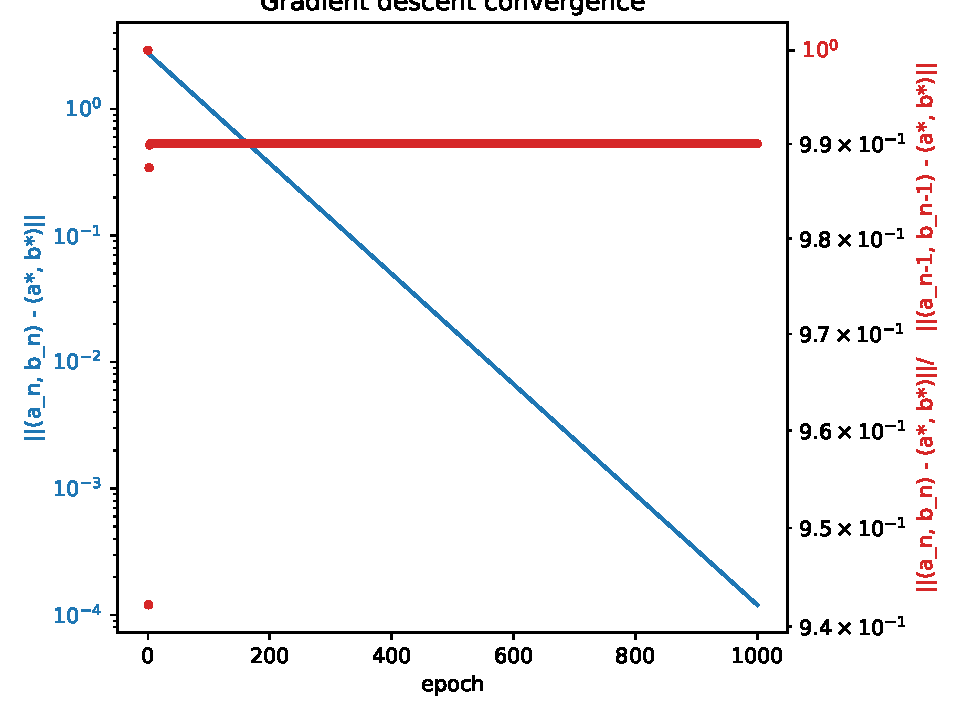
\includegraphics{Homework1/ex2b.pdf}
    \caption{Gradient descent convergence}
\end{figure}
The convergence rate of momentum and Nesterov methods are hard to find on the plot, but they are faster than regular gradient descent.
It takes around 600 epochs to converge to \(10^{-15}\) float-point accuracy, while regular gradient descent takes 1000 epochs to reach \(10^{-4}\).
\begin{figure}[htbp]
    \centering
    \begin{subfigure}[t]{0.68\textwidth}
        \centering
        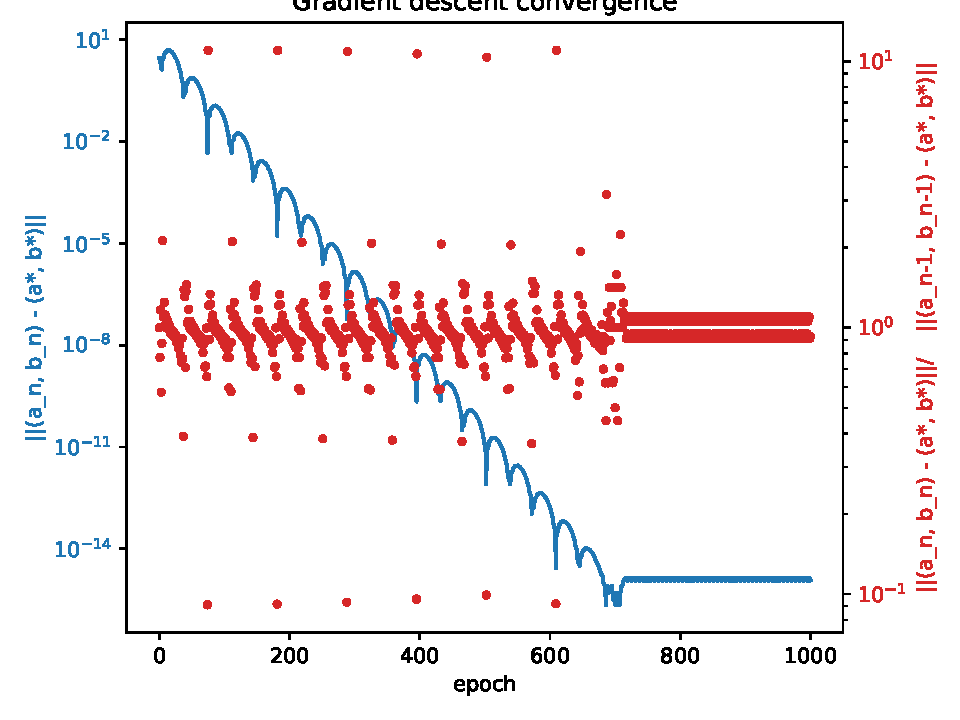
\includegraphics[width=\textwidth]{Homework1/ex2cm.pdf}
        \caption{Convergence of momentum method}
    \end{subfigure}\vspace{10pt}
    \begin{subfigure}[t]{0.68\textwidth}
        \centering
        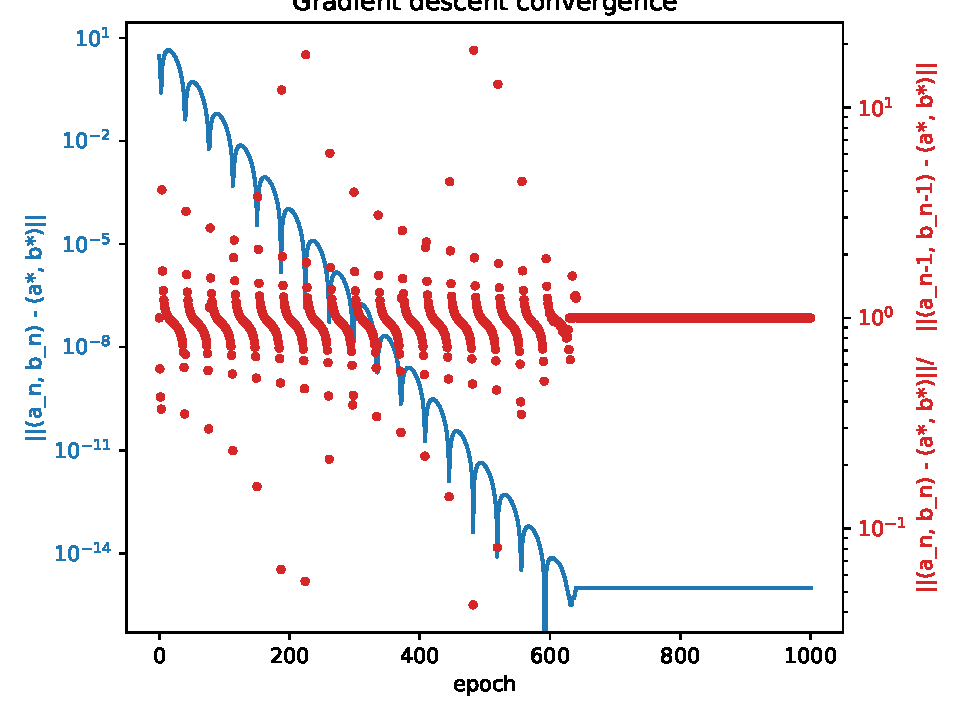
\includegraphics[width=\textwidth]{Homework1/ex2cn.pdf}
        \caption{Convergence of Nesterov method}
    \end{subfigure}
\end{figure}
\paragraph{(extra)}
Other gradient descent methods are implemented in PyTorch.
Most of the errors don't decay as fast as the regular gradient descent.
This is because they are designed for highly non-convex loss functions (to escape from local optimum), while the MSE loss function for linear regression is convex.
\begin{figure}[htbp]
    \centering
    \begin{subfigure}[t]{0.48\textwidth}
        \centering
        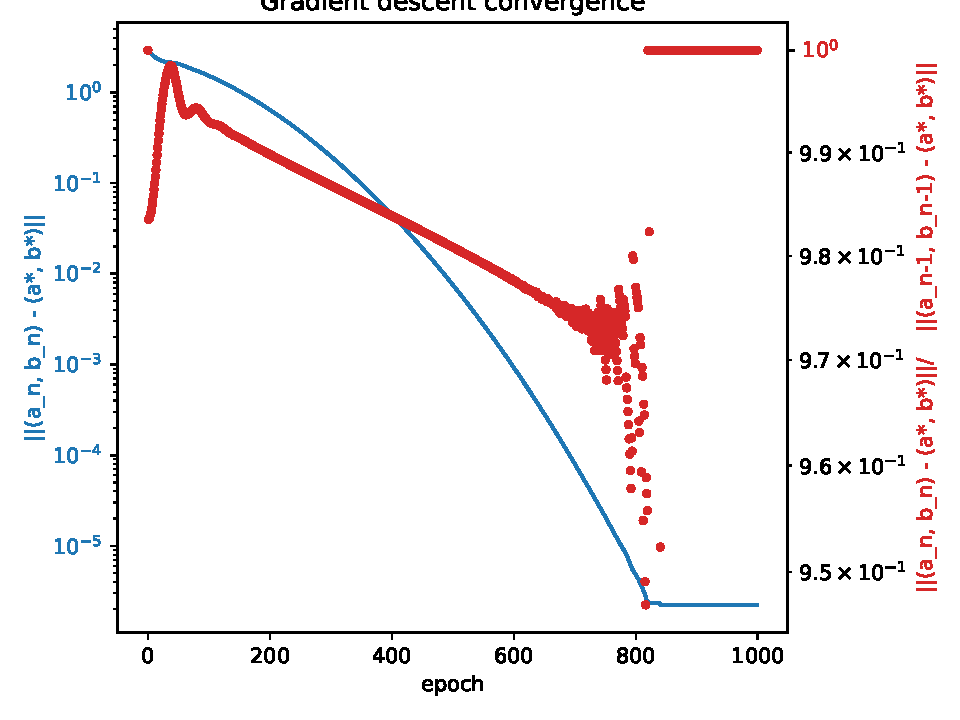
\includegraphics[width=\textwidth]{Homework1/ex2x1.pdf}
        \caption{Adam}
    \end{subfigure}
    \begin{subfigure}[t]{0.48\textwidth}
        \centering
        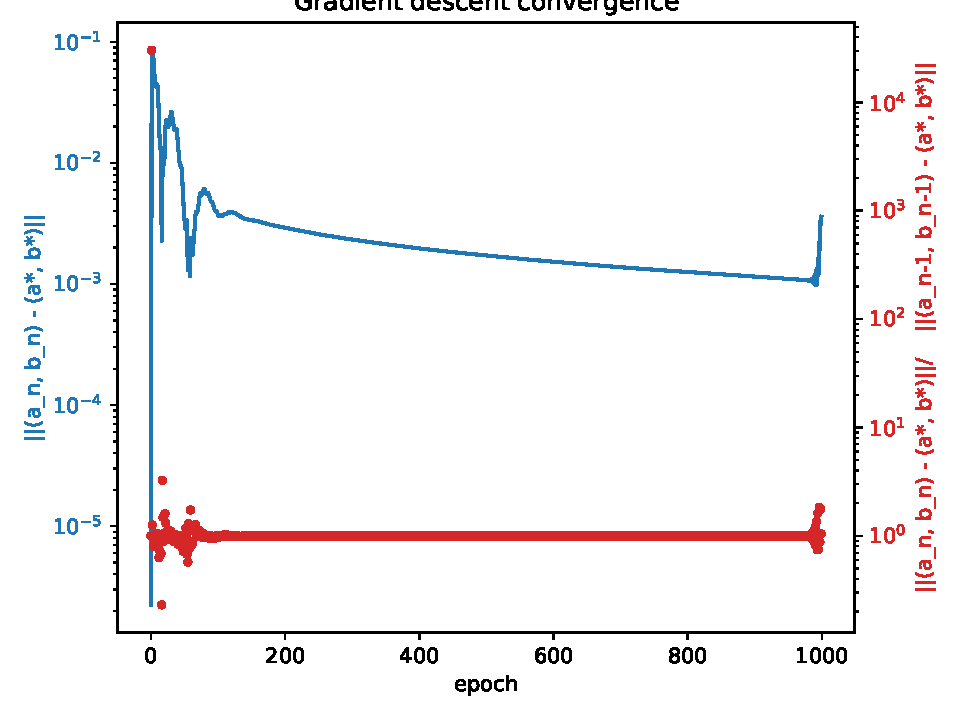
\includegraphics[width=\textwidth]{Homework1/ex2x2.pdf}
        \caption{AdamW}
    \end{subfigure}
    \centering
    \begin{subfigure}[t]{0.48\textwidth}
        \centering
        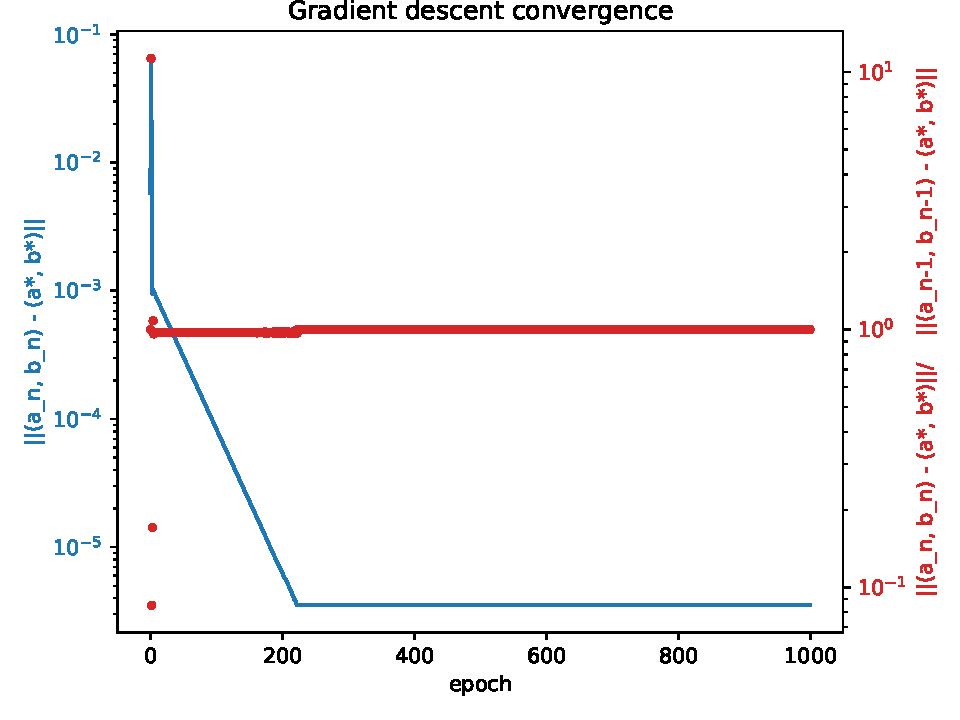
\includegraphics[width=\textwidth]{Homework1/ex2x3.pdf}
        \caption{Adagrad}
    \end{subfigure}
    \begin{subfigure}[t]{0.48\textwidth}
        \centering
        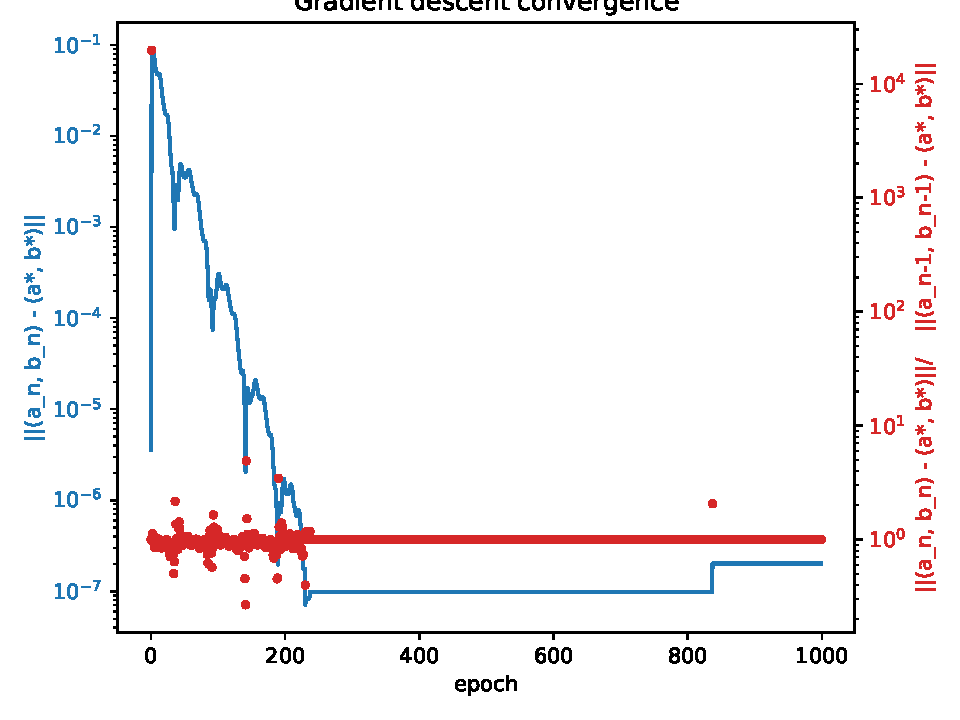
\includegraphics[width=\textwidth]{Homework1/ex2x4.pdf}
        \caption{Adamax}
    \end{subfigure}
    \centering
    \begin{subfigure}[t]{0.48\textwidth}
        \centering
        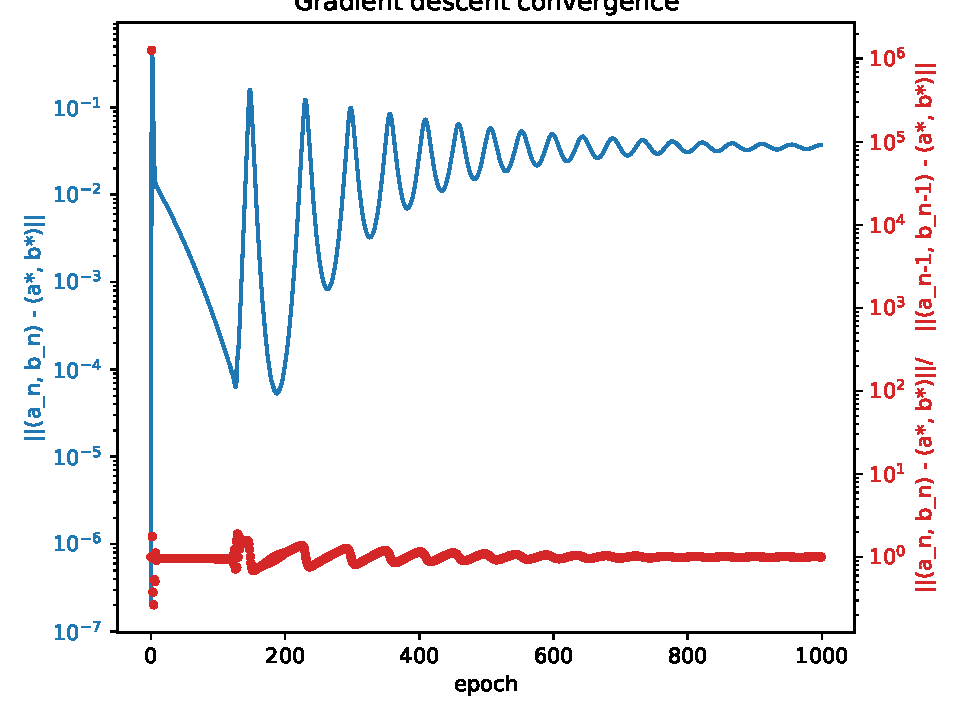
\includegraphics[width=\textwidth]{Homework1/ex2x5.pdf}
        \caption{RMSprop}
    \end{subfigure}
    \begin{subfigure}[t]{0.48\textwidth}
        \centering
        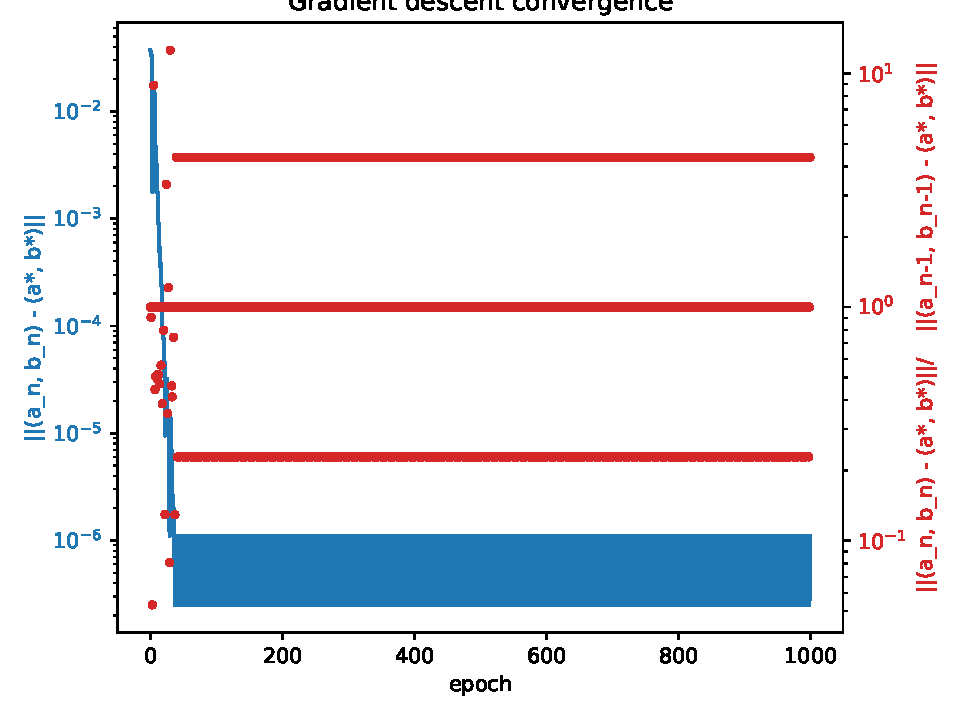
\includegraphics[width=\textwidth]{Homework1/ex2x6.pdf}
        \caption{Rprop}
    \end{subfigure}
\end{figure}
\inputminted[breaklines=true, linenos=true]{python}{./Homework1/ex2.py}
\newpage

\subsection{Classification}
\begin{figure}[htbp]
    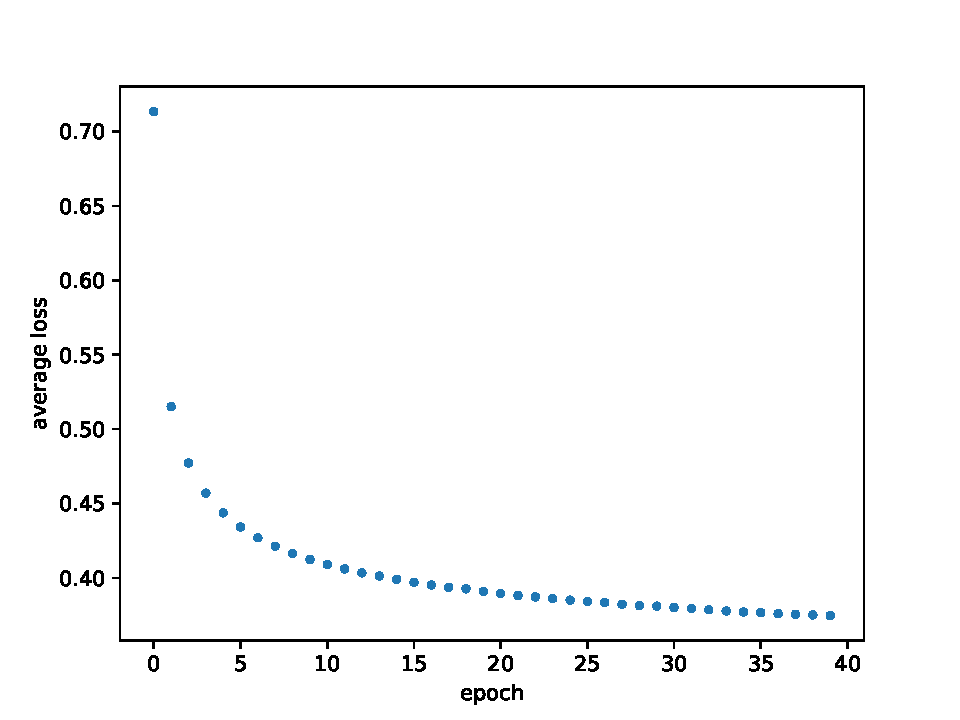
\includegraphics{Homework1/ex3b.pdf}
    \caption{Evolution of the loss}
\end{figure}
\foreach\x in {0,...,4}
{
\begin{figure}
\begin{center}
    \foreach \i in {{\number\numexpr2*\x\relax},{\number\numexpr2*\x+1\relax}}
    {
        \begin{subfigure}[p]{0.8\textwidth}
            \includegraphics[width=\textwidth]{Homework1/ex3c\i.pdf}
        \end{subfigure}
    }
\end{center}
\end{figure}
\clearpage
}
\inputminted[breaklines=true, linenos=true]{python}{./Homework1/ex3.py}
\newpage

\section{Homework}
\subsection{Two-layers neural networks}
\paragraph{(a)}
Consider the following parameters
\[ W_1=\begin{bmatrix} 3 & 5 \\ 1 & 3 \end{bmatrix} \hspace{1em}
   b_1=\begin{bmatrix} 5 \\ 1 \end{bmatrix} \hspace{1em}
   W_2=\begin{bmatrix} 1 & 0 \\ 0 & 3 \end{bmatrix} \hspace{1em}
   b_2=\begin{bmatrix} 0 \\ 1 \end{bmatrix}. \]
Plug in \(f(x)=b_2+W_2\left(\sigma(b_1+W_1 x) \right)\), we get
\[ f(x_1)=\begin{bmatrix} 3 \\ 1 \end{bmatrix} \hspace{1em}
   f(x_2)=\begin{bmatrix} 2 \\ 1 \end{bmatrix} \hspace{1em}
   f(x_3)=\begin{bmatrix} 10 \\ 13 \end{bmatrix} \hspace{1em}
   f(x_4)=\begin{bmatrix} 0 \\ 1 \end{bmatrix}. \]
\paragraph{(b)}
The result two-layer neural network after training has parameters
\[ W_1=\begin{bmatrix} -0.6996 & 5.3405 \\ -0.3927 & 4.0549 \end{bmatrix} \hspace{5pt}
   b_1=\begin{bmatrix} 5.6579 \\ 0.1506 \end{bmatrix} \hspace{5pt}
   W_2=\begin{bmatrix} 1.2514 & -0.4970 \\ -0.2514 & 3.4970 \end{bmatrix} \hspace{5pt}
   b_2=\begin{bmatrix} -1.0276 \\ 2.0276 \end{bmatrix}. \]
The classification accuracy is 92.5\%.
\begin{figure}[htbp]
    \centering
    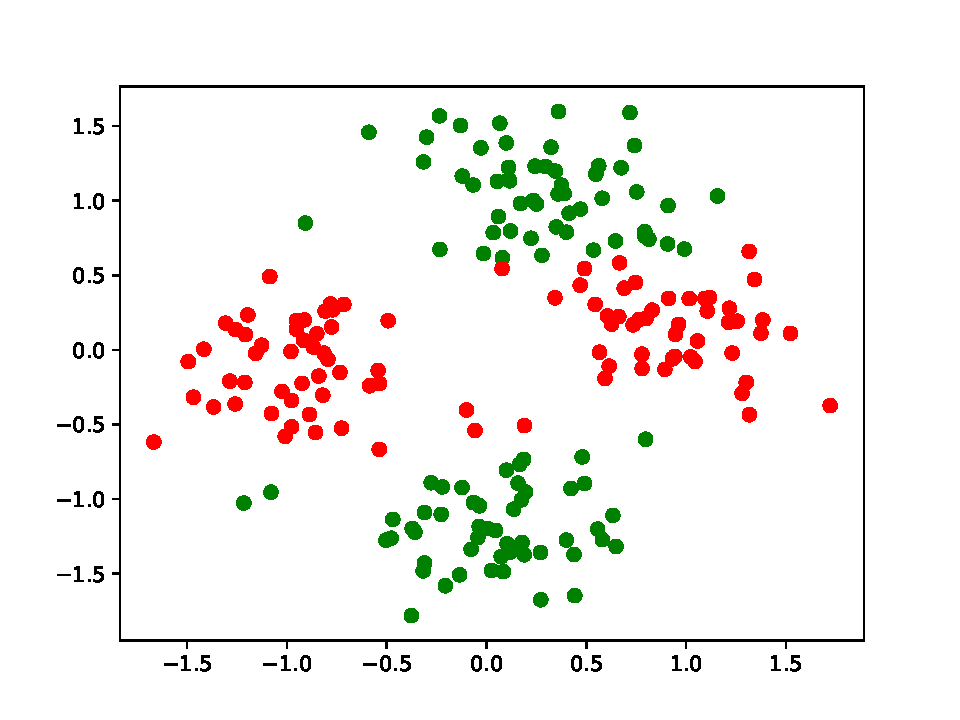
\includegraphics[scale=0.9]{Homework2/ex1b.pdf}
    \caption{Trained two-layer neural network prediction}
\end{figure}
\inputminted[breaklines=true, linenos=true]{python}{./Homework2/ex1.py}
\newpage

\subsection{Neural networks dense in continuous functions}
\paragraph{(a)}
In this case, \(W_1, W_2\in\mathbb{R}^{1\times1}\) (so we write \(w_1, w_2\)), \(b_1,b_2\in\mathbb{R}^1\), and
\[ f(x) = b_2 + w_2 \sigma(b_1 + w_1 x). \]
Then plug in \(x=0\) and \(x=1\) to get following system of equations
\begin{align*}
    y_0 &= b_2 + w_2 \sigma(b_1+w_1\cdot0), \\
    y_1 &= b_2 + w_2 \sigma(b_1+w_1\cdot1).
\end{align*}
We can choose \(b_2 = \min\{y_0, y_1\}\) and \(w_2=1\), then the equations simplify to
\begin{align*}
    \sigma(b_1) &= y_0 - \min\{y_0, y_1\} = \max\{0, y_0-y_1\} = \sigma(y_0-y_1), \\
    \sigma(b_1 + w_1) &= y_1 - \min\{y_0, y_1\} = \max\{y_1-y_0, 0\} = \sigma(y_1-y_0).
\end{align*}
So we can choose \(w_1=y_1-y_0\) and then \(b_1=\sigma(y_0-y_1)\).
To write them together,
\[ f(x) = \min\{y_0, y_1\} + \sigma[\sigma(y_0-y_1)+(y_1-y_0)x]. \]
\paragraph{(b)}
Consider \(m=3\) so that
\[ W_1=\begin{bmatrix} w_{11} \\ w_{12} \\ w_{13} \end{bmatrix} \hspace{1em}
   b_1=\begin{bmatrix} b_{11} \\ b_{12} \\ b_{13} \end{bmatrix} \hspace{1em}
   W_2=\begin{bmatrix} w_{21} \\ w_{22} \\ w_{23} \end{bmatrix} \hspace{1em}
   b_2=\begin{bmatrix} b_{21} \\ b_{22} \\ b_{23} \end{bmatrix}. \]
Then the conditions give the following equations
\begin{align*}
    f(0)=y_0 &\implies& y_0 - b_2 &= w_{21}\sigma(b_{11}) + w_{22}\sigma(b_{12}) + w_{23}\sigma(b_{13}) \\
    f(1/2)=y_1 &\implies& y_1 - b_2 &= w_{21}\sigma(b_{11}+w_{11}/2) + w_{22}\sigma(b_{12}+w_{12}/2) + w_{23}\sigma(b_{13}+w_{13}/2) \\
    f(1)=y_2 &\implies& y_2 - b_2 &= w_{21}\sigma(b_{11}+w_{11}) + w_{22}\sigma(b_{12}+w_{12}) + w_{23}\sigma(b_{13}+w_{13}),
\end{align*}
which is equivalent to
\[ \begin{bmatrix} \sigma(b_{11}) & \sigma(b_{12}) & \sigma(b_{13}) \\
    \sigma(b_{11}+w_{11}/2) & \sigma(b_{12}+w_{12}/2) & \sigma(b_{13}+w_{13}/2) \\ 
    \sigma(b_{11}+w_{11}) & \sigma(b_{12}+w_{12}) & \sigma(b_{13}+w_{13}) \end{bmatrix}
    \begin{bmatrix} w_{21} \\ w_{22} \\ w_{23} \end{bmatrix} = 
    \begin{bmatrix} y_0-b_2 \\ y_1-b_2 \\ y_2-b_2 \end{bmatrix}. \]
So we have some freedom to choose \(W_1\) and \(b_1, b_2\) without making the matrix singular.
\[ W_1=\begin{bmatrix} 4 \\ 2 \\ 6 \end{bmatrix} \hspace{1em}
   b_1=\begin{bmatrix} -1 \\ 2 \\ 3 \end{bmatrix} \hspace{1em}
   b_2=\begin{bmatrix} 0 \\ 0 \\ 0 \end{bmatrix}. \]
Then the system becomes
\[ \begin{bmatrix} 0 & 2 & 3 \\ 1 & 3 & 6 \\ 3 & 4 & 9 \end{bmatrix}W_2 = \begin{bmatrix} y_0 \\ y_1 \\ y_2 \end{bmatrix}. \]
The LHS matrix has determinant 3, so \(W_2\) has a unique solution.
\paragraph{(c)}
We can choose \(m=N+1\) so that
\[ \begin{bmatrix} \sigma(b_{11}+w_{11}x_0) & \cdots & \sigma(b_{1m}+w_{1m}x_0) \\
    \sigma(b_{11}+w_{11}x_1) & \ddots & \sigma(b_{1m}+w_{1m}x_1) \\ 
    \vdots & \cdots & \vdots \\
    \sigma(b_{11}+w_{11}x_{N}) & \cdots & \sigma(b_{1m}+w_{1m}x_N) \end{bmatrix}
    \begin{bmatrix} w_{21} \\ \vdots \\ w_{2m} \end{bmatrix} = 
    \begin{bmatrix} y_0-b_2 \\ \vdots \\ y_N-b_2 \end{bmatrix} \]
can have a unique solution for \(W_2\) by carefully choosing \(W_1\) and \(b_1\).
\paragraph{(Extra)}
Notice that both \(f\) and \(g\) are continuous on the compact interval \([0, 1]\), so they are uniformly continuous.
So for any \(\epsilon>0\) there exists a partition \((x_n)_{n=0}^{N}\subset[0, 1]\) (WLOG sorted as \(0\leq x_0<x_1<\cdots<x_N\leq1\)) with
\[ \|(x_n)_{n=0}^{N}\|:= \max_{n\in[N]}|x_{n}-x_{n-1}| < \min\{\delta_1, \delta_2\}, \]
where \(\delta_1, \delta_2\) are defined by
\begin{align*}
    \forall n\in[N],& |x-x_n|<\delta_1 \implies |g(x)-g(x_n)|<\frac{\epsilon}{3},\\
    \forall n\in[N],& |x-x_n|<\delta_2 \implies |f(x)-f(x_n)|<\frac{\epsilon}{3},
\end{align*}
Then for all \(x\in[0, 1]\), there is \(n\in[N]\) such that \(|x-x_n|<\min\{\delta_1, \delta_2\}\) and thus
\[ |f(x)-g(x)| \leq |f(x)-f(x_n)+g(x_n)-g(x)| \leq |f(x)-f(x_n)|+|g(x_n)-g(x)| < \frac{\epsilon}{3}+\frac{\epsilon}{3}, \]
where we use the property \(f(x_n)=g(x_n)\) on the partition grids.
\newpage

\subsection{Convolutional neural networks}
The beginning layers are adapted from VGG11.
A few layers are removed so it's called VGG8.
The test accuracy (on 10000 images) after training 10 epochs is 85.28\%.
\inputminted[breaklines=true, linenos=true]{python}{./Homework2/ex3.py}
\newpage
\end{comment}

\section{Homework}
\subsection{n-gram models}
\inputminted[breaklines=true, linenos=true]{python}{./Homework3/ex1.py}
\paragraph{(a)}
The total number of words is \(T=136312\).
\paragraph{(b)}
The 5 most common words with at least 8 characters are
(certainly, 235), (knowledge, 152), (injustice, 111), (therefore, 109), (question, 99).
\paragraph{(d)}
The perplexity of the bi-gram model is \(PP=37.89928782828084\).
\newpage

\subsection{Recurrent neural networks}
\inputminted[breaklines=true, linenos=true]{python}{./Homework3/ex2.py}
\paragraph{(a)}
The predicted characters are `hello'.
\begin{align*}
    \mathbf{y}_1&=\begin{bmatrix} 1.5232 &  1.1424 & -0.7616 & -0.3808\end{bmatrix}\\
    \mathbf{y}_2&=\begin{bmatrix} 0.7087 &  0.8257 &  0.2340 & -0.4713\end{bmatrix}\\
    \mathbf{y}_3&=\begin{bmatrix}-0.2096 &  0.1031 &  0.6255 & -0.2079\end{bmatrix}\\
    \mathbf{y}_4&=\begin{bmatrix}-0.8934 & -0.4887 &  0.8095 &  0.0420\end{bmatrix}\\
    \mathbf{y}_5&=\begin{bmatrix}-1.0946 & -0.9446 &  0.3000 &  0.3973\end{bmatrix}
\end{align*}
\paragraph{(b)}
This is obtained by training the RNN with target being `olleh'.
\begin{align*}
    A &= \begin{bmatrix}
         0.9330 & -2.4132 & -0.1931 &  2.2354 \\
        -1.5668 &  3.1719 &  0.4204 &  0.2432
    \end{bmatrix} \\
    R &= \begin{bmatrix}
         0.5683 &  0.3168 \\ -0.9781 &  2.0761
    \end{bmatrix} \\
    B &= \begin{bmatrix}
         2.3623 &  0.8963 \\ -1.4019 &  1.6015 \\
        -3.5722 &  0.9827 \\ 1.8588 & -1.5987
    \end{bmatrix}
\end{align*}
\newpage

\subsection{Vanishing/exploding gradient}
\paragraph{(a)}
By (vector-valued function) chain rule,
\[ D_\mathbf{h}(\mathbf{h}\mapsto\sigma(R\mathbf{h}+A\mathbf{x}_t))=\sigma'(R\mathbf{h}+A\mathbf{x}_t)R, \hspace{1em} \mathbf{h},\mathbf{x}_t\in\mathbb{R}^d, R,A\in\mathbb{R}^{d\times d}, \sigma'\in\mathbb{R}^{d}\to\mathbb{R}^{d\times d}. \]
so
\[ D_{\mathbf{x}_1}\mathbf{y}_t =D_{\mathbf{h}_t}\mathbf{y}_t \left(\prod_{k=2}^{t}D_{\mathbf{h}_{k-1}}\mathbf{h}_k \right) D_{\mathbf{x}_1}\mathbf{h}_1=B\left( \prod_{k=2}^{t} \sigma'(R\mathbf{h}_{k-1}+A\mathbf{x}_{k})R \right)\sigma'(R\mathbf{h}_0+A\mathbf{x}_1)A. \]
By product triangle inequality of matrix norm,
\begin{align*}
\|D_{\mathbf{x}_1}\mathbf{y}_t\| &\leq \|B\| \left( \prod_{k=2}^{t} \|\sigma'(R\mathbf{h}_{k-1}+A\mathbf{x}_{k})\|\cdot\|R\| \right)\|\sigma'(R\mathbf{h}_0+A\mathbf{x}_1)\|\cdot\|A\|\\
&=\|B\|\left( \prod_{k=1}^{t} \|\sigma'(R\mathbf{h}_{k-1}+A\mathbf{x}_{k})\| \right)\|R\|^{t-1}\cdot\|A\|.
\end{align*}
\paragraph{(b)}
For \(\mathbf{x}_1=(0, 0)\) and \(\mathbf{x}_1^\varepsilon=(\varepsilon, -\varepsilon)\),
\begin{align*}
\|\mathbf{y}_{30}-\mathbf{y}_{30}^\varepsilon\|_2(10^{-4},\cdots,10^{-9})= (1.2129358, 1.0311685, 1.7903578\times10^{-1},\\ 1.8076686\times10^{-2}, 1.8078436\times10^{-3}, 1.8078458\times10^{-4}).
\end{align*}
\begin{figure}[htbp]
    \centering
    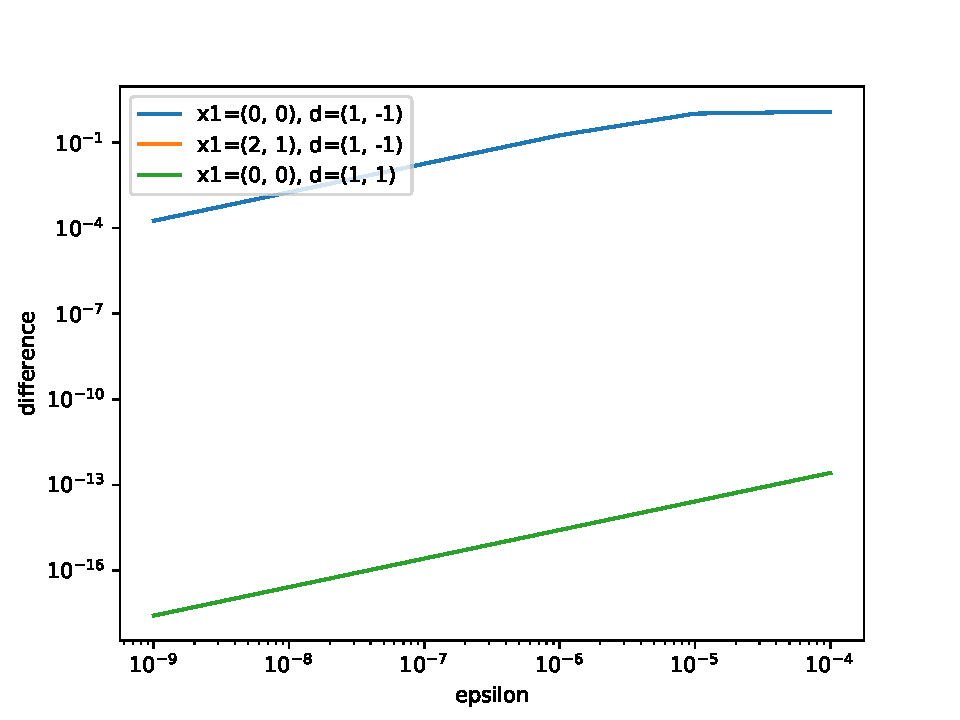
\includegraphics[scale=0.9]{Homework3/ex3.pdf}
    \caption{perturbation effect (\(\mathbf{x}_1=(2, 1)\) invisible)}
\end{figure}
\paragraph{(c)}
For \(\mathbf{x}_1=(2, 1)\) and \(\mathbf{x}_1^\varepsilon=(2+\varepsilon, 1-\varepsilon)\),
\[ \|\mathbf{y}_{30}-\mathbf{y}_{30}^\varepsilon\|_2(10^{-4},\cdots,10^{-9})=(0, 0, 0, 0, 0, 0) \times10^{-16}, \]
where \(10^{-16}\) is from the machine epsilon of the floating point arithmetic.
This is because \(\sigma'\) is small near \(\mathbf{x}_1\):
\[ \sigma'(R\mathbf{h}_0+A\mathbf{x}_1)=\sigma'(\mathbf{x}_1)=\begin{bmatrix} 1-\tanh^2(2) & 0 \\ 0 & 1-\tanh^2(1) \end{bmatrix} \approx \begin{bmatrix}0.07 & 0 \\ 0 & 0.42 \end{bmatrix}. \]
The rest of the \(\sigma'\) are also small near \(R\mathbf{h}_k\), so the bound on \(D_{\mathbf{x}_1}\mathbf{y}_t\) is nearly 0.
\paragraph{(Extra)}
This is because \(\mathbf{x}_1^\varepsilon=(\varepsilon, -\varepsilon)\) is an eigenvector of \(R\) with corresponding eigenvalue \(\lambda_1=\frac{3}{2}>1\), so the initial perturbation get amplified; while \(\mathbf{x}_1^\varepsilon=(\varepsilon, \varepsilon)\) is another eigenvector of \(R\) with corresponding eigenvalue \(\lambda_2=-\frac{1}{2}>-1\), so the initial perturbation is compressed.
For a random perturbation \(\mathbf{x}_1\in\mathbb{R}^2\), if it is amplified by \(R\), i.e.,
\[ \mathbf{x}_1\in\{(x_1, x_2): x_1 x_2 < 0 \}\subset\mathbb{R}^2, \]
then the perturbation has a large effect (expanded gradient).
Otherwize,
\[ \mathbf{x}_1\in\{(x_1, x_2): x_1 x_2 > 0 \}\subset\mathbb{R}^2 \]
leads to a small effect due to vanishing gradient.
\inputminted[breaklines=true, linenos=true]{python}{./Homework3/ex3.py}

\end{document}